\chapter{SynCaps}

\label{chap:SynCaps}

SynCaps is an older card sorting tool that is not available online. It
is only usable as an offline Windows program that needs to be 
installed locally. Since 2018 the full package is offered free of 
charge and can be downloaded. It is not trivial to use and requires 
some time spent with the provided documentation videos. Its workflow
is dated and requires some getting used to~\parencite{SynCaps}.

As the tool does not offer any card sorting capabilities, this needs
to be taken care of in some other way. Originally SynCaps was intended
to be used in cooperation with paper card sorting. After the
experiment was done one can import the data into SynCaps and analyze
it. Nowadays it is also very easy to use other card sorting tools and
then import the data into SynCaps for analytics.

\begin{figure}[tp] 
\centering
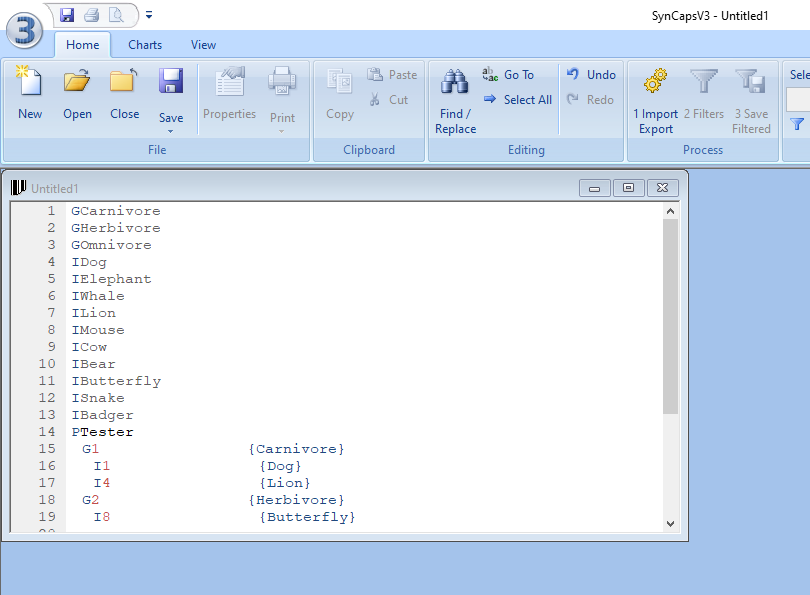
\includegraphics[keepaspectratio,width=\linewidth,height=\halfh]{images/syncaps-sorting.png}
\caption[SynCaps Application] { This is the base view within SynCaps.
All input data is handled within a .txt file as shown in the screenshot.
\imgcredit{Screenshot was captured by Christopher Oser using
\textcite{SynCaps}.} }
\label{fig:SynCaps1}
\end{figure}

\section{Business Model}
As mentioned earlier SynCaps is totally free of charge. There are no
additional features to be unlocked by a paywall. Previously other 
restrictions applied, but since 2018 the tool is not only free of
charge, but also licensing free.

Being an offline program, there is also no need for an account. Any 
data is saved locally and needs to be manually moved to be accessed in
other environments.

\section{Card Sorting}
SynCaps does not provide any card sorting capabilities. It is intended
to be used with paper card sorting or other tools. For paper card
sorting, it provides an option to assign barcodes to cards, for easier
importing of the results after the experiment.

\section{Analytics}
This is were this tool shines. When analyzing results from card
sorting experiments, the options are quite numerous, not so say
overwhelming. Before any analytics, there is the possibility for
data preparation. Users can be singled out, cards as well as categories
can be merged and lots more.

Once the data has been prepared the results can be analyzed within 5
different charts that can be further customized. These charts are made
up of clusterings and dendrograms with different inputs. These charts
are somewhat interactive, as a click on a datapoint will reveal more
information about it, but that is also where the interactivity ends.

The features are summarized in Table~\ref{tab:features-SynCaps}.

\begin{figure}[tp] 
\centering
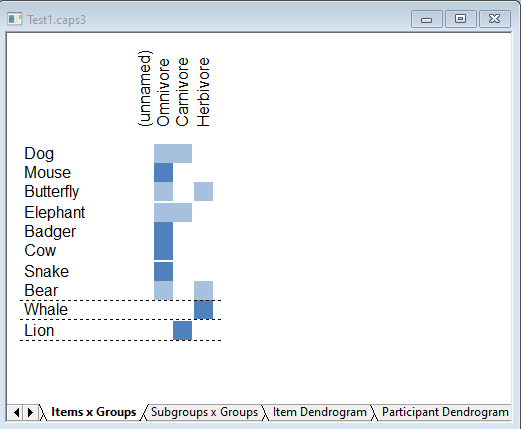
\includegraphics[keepaspectratio,width=\linewidth,height=\halfh]{images/syncaps-diagram-1.png}
\caption[SynCaps Clustering] { This screenshot shows a Cards x Groups
visualization used for analytics.
\imgcredit{Screenshot was captured by Christopher Oser using
\textcite{SynCaps}.} }
\label{fig:SynCaps2}
\end{figure}

\begin{figure}[tp] 
\centering
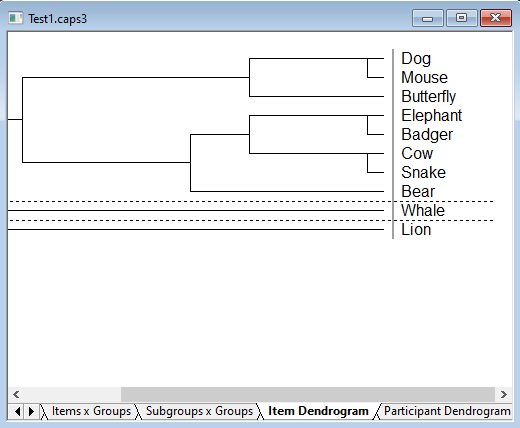
\includegraphics[keepaspectratio,width=\linewidth,height=\halfh]{images/syncaps-diagram-2.png}
\caption[SynCaps Dendrogram] { This screenshot shows a Cards 
dendrogram used for analytics.
\imgcredit{Screenshot was captured by Christopher Oser using
\textcite{SynCaps}.} }
\label{fig:SynCaps3}
\end{figure}

\begin{table}[tp]
\centering
\begin{tabularx}
{\linewidth}{|l|X|}
\hline \textbf{Feature/Characteristic} & \textbf{Availability in SynCaps} \\ 
\hline Card Sorting & None. Paper Cards or other tools needed. \\ 
\hline Card Limit & None. \\
\hline Participant Limit & None. \\
\hline Analytics & Analytics in 5 semi-interactive
charts made up of clusterings and dendrograms \\ 
\hline Documentation & Some dated videos. \\
\hline Business Model & Free. \\
\hline Import formats & .csv, .txt or paste\\ 
\hline Export formats & .csv \\ 
\hline Sub-Categories & Yes, sub-categories are supported \\ 
\hline Playback of user-sessions & No. \\ 
\hline Data preparation & Extensive options from user exclusion to
card merging. \\ 
\hline
\end{tabularx} 
\caption[Feature summary of SynCaps] 
{ 
This table summarizes all the features and characteristics of SynCaps
to provide an easy to read overview.
}
\label{tab:features-SynCaps}
\end{table}


\section{Summary \& Ratings} SynCaps is a solid analytics tool if you
can get past its workflow and learning curve. The videos offered as
documentation, but are not fun to watch to say the least. It offers
many data preparation options and enables efficient evaluation of
results with its many semi-interactive  visualizations.

It is always necessary to pair SynCaps with either physical paper card
sorting or another tool to perform the actual card sorting. If this is
an option, then SynCaps can be very handy for analyzing.

For a quick overview and to make it easier to compare to other tools
in this paper, we agreed on 4 ratings for the tool. The ratings can be
found in Table~\ref{tab:rating-SynCaps} and range from 0-5.

\begin{table}[tp] 
\centering 
\begin{tabularx}{\linewidth}{|X|X|X|X|X|}
\hline
Simplicity & Documentation & Features & Business Model & Average \\ 
\hline 
1 & 2 & 4 & 5 & 3.0 \\ 
\hline 
\end{tabularx} 
\caption[Ratings for SynCaps] {
Ratings for SynCaps including the average rating.
} 
\label{tab:rating-SynCaps}
\end{table}